\documentclass{report}
\usepackage[utf8]{inputenc}

\title{”Vienkāršu elektrisku shēmu modelēšana”}
\author{mark-voroncov }
\date{April 2018}

\usepackage{graphicx}
\graphicspath{{pictures/}}
\DeclareGraphicsExtensions{.pdf,.png,.jpg}

\begin{document}

\maketitle

\chapter{Teorētiskā daļa}
\section{Ķēdes aprēķins}
Sprieguma avota V1 sprieguma vērtību U (Voltos) izvēlietieshttp daļskaitli, kas būtu Jūsu apliecības pēdējie trīs cipari dalīti ar 10. Piemēram. ‘171REB150’ nozīmē V1 = 15.0 (Volti), R1 ir apliecības pēdējo 3 ciparu otrais numurs+1, R2 ir apliecības numura pēdējais cipars +1. Piemēram, ja Jūsu apliecības numurs ir ‘171REB150’ tad ‘R1=6’, ‘R2=1’.  


\begin{tabular}{|c|c|}
\hline
     R1 & 6 \\ \hline
     R2 & 1 \\ \hline 
     V1 & 15.0 \\ \hline
     Ur2 &  \\ \hline
     Ur1 &  \\
\hline
\end{tabular}

\chapter{Praktiskā daļa}
\section{Darbs ar GEDA programmām}
\subsection{darbs ar gschem}

\begin{figure}[h]
\center{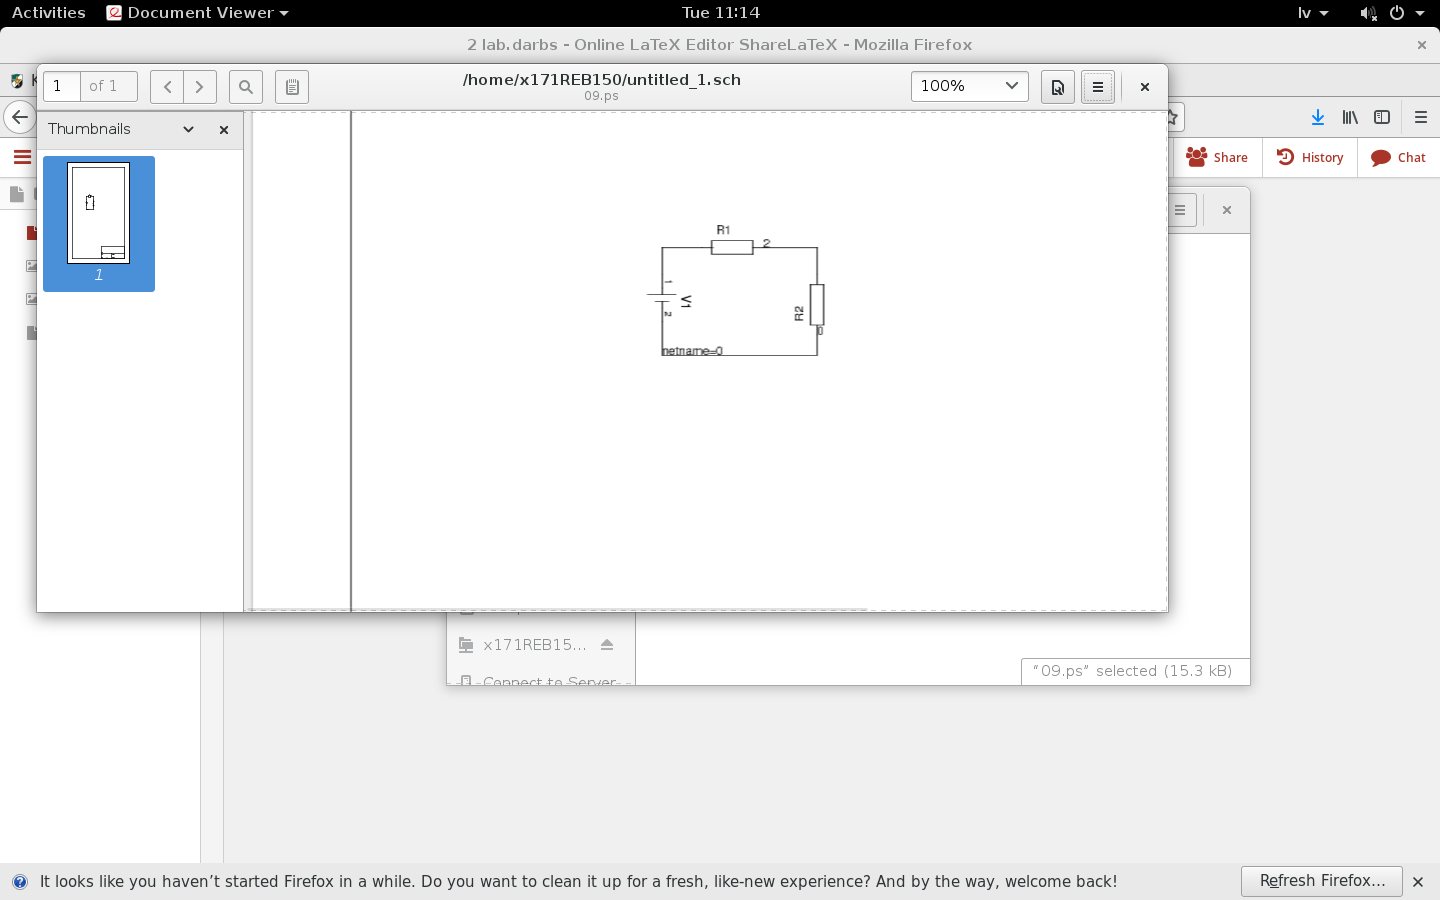
\includegraphics[scale=0.250]{40}}
\caption{Тестовый рисунок "Grafiks ar visiem pz"}
\label{fig:image}
\end{figure}

\subsection{darbs ar ngspice}
\begin{figure}[h]
\center{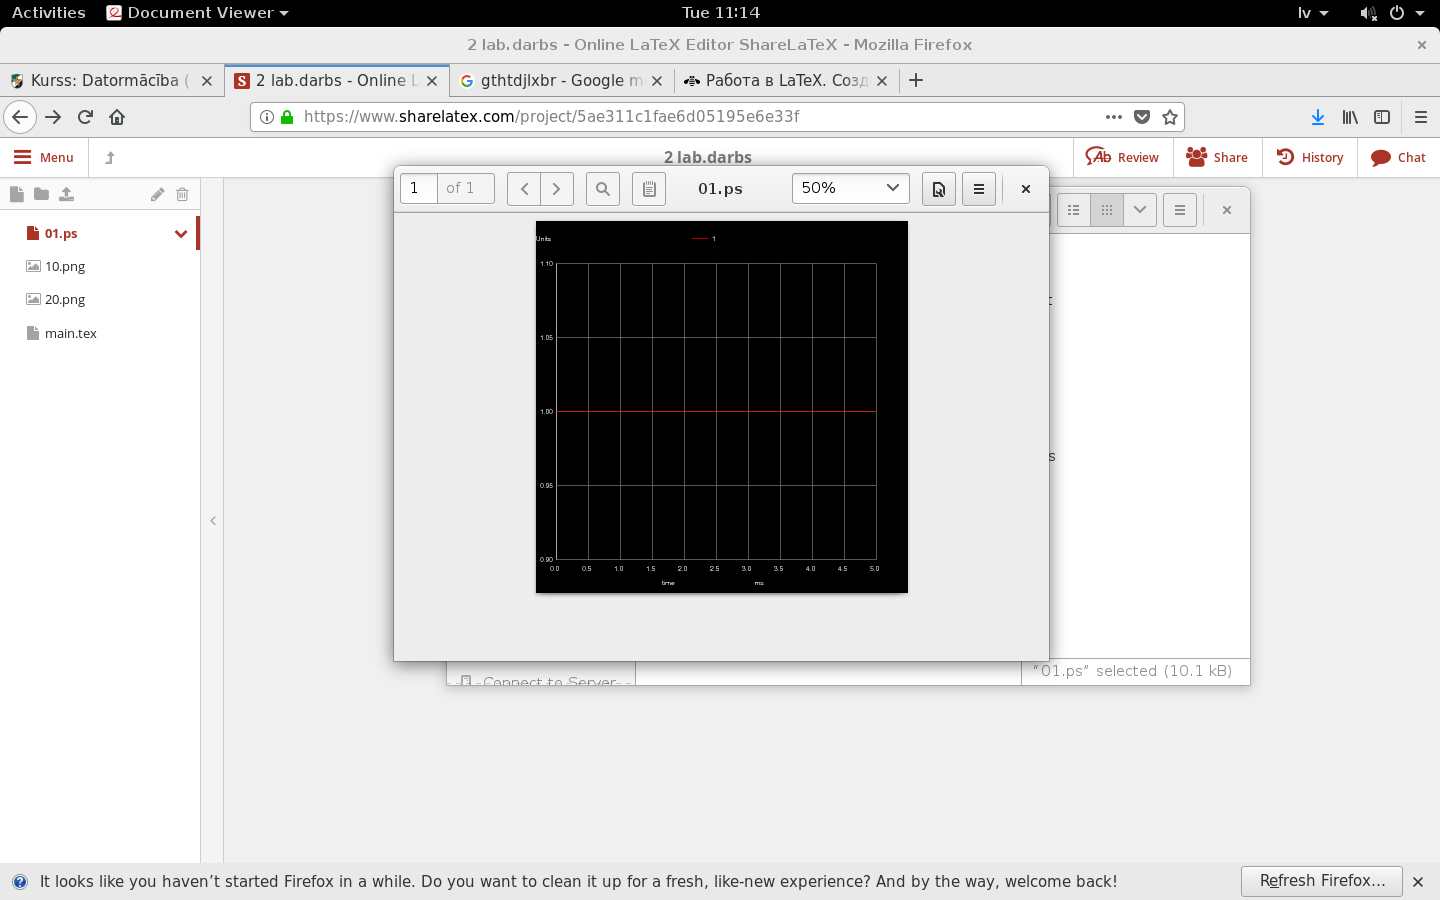
\includegraphics[scale=0.250]{30.png}}
\center{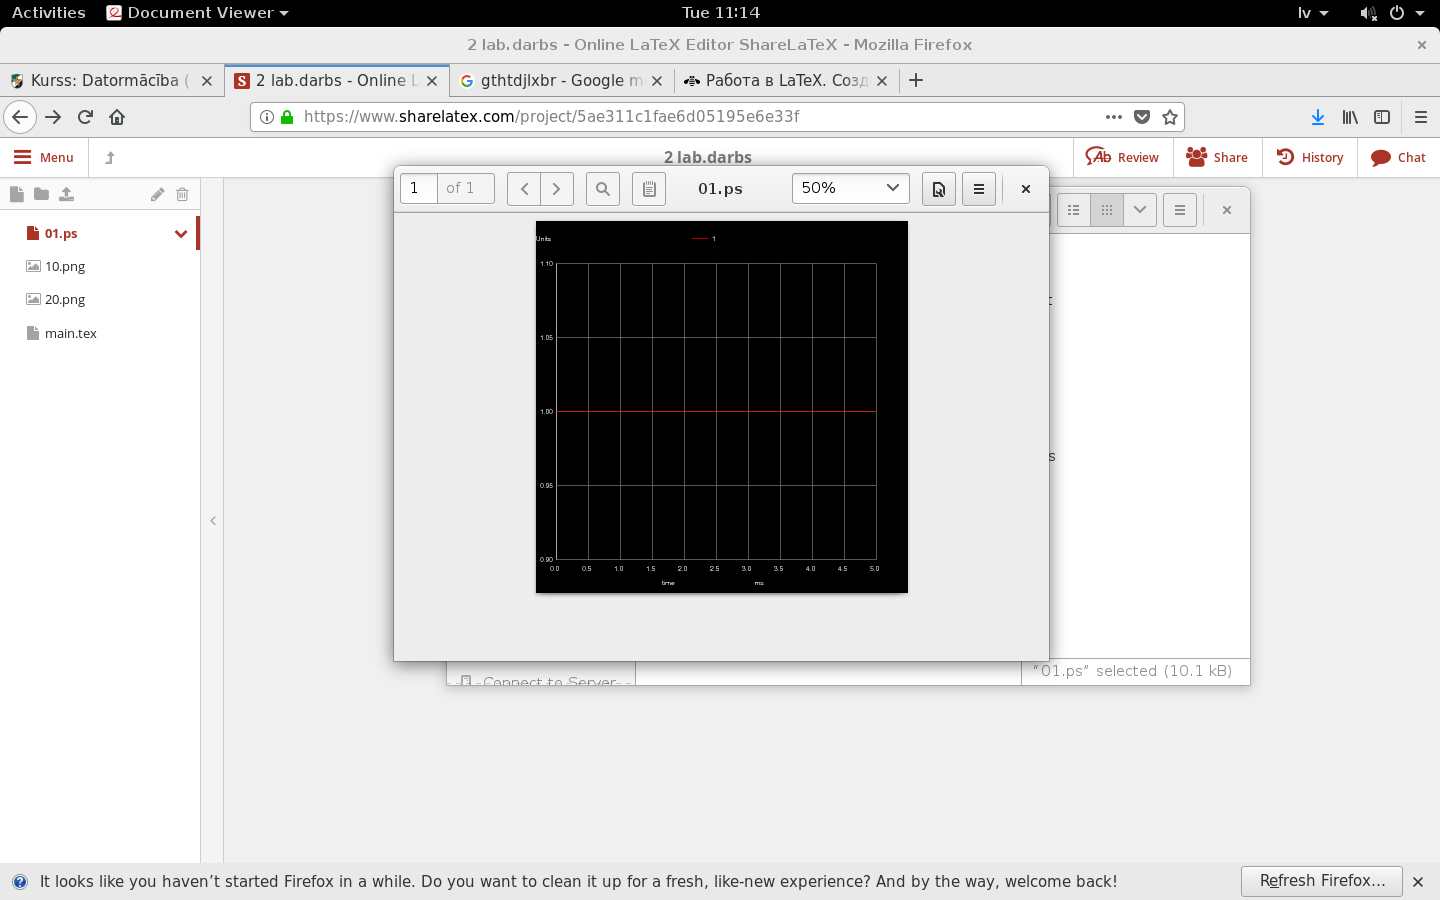
\includegraphics[scale=0.250]{30.png}}
\caption{Тестовый рисунок "Darbs ar programmu ngspice"}
\label{fig:image}
\end{figure}


\subsection{‘Darbs ar QUCS programmām}
\begin{figure}[h]
\center{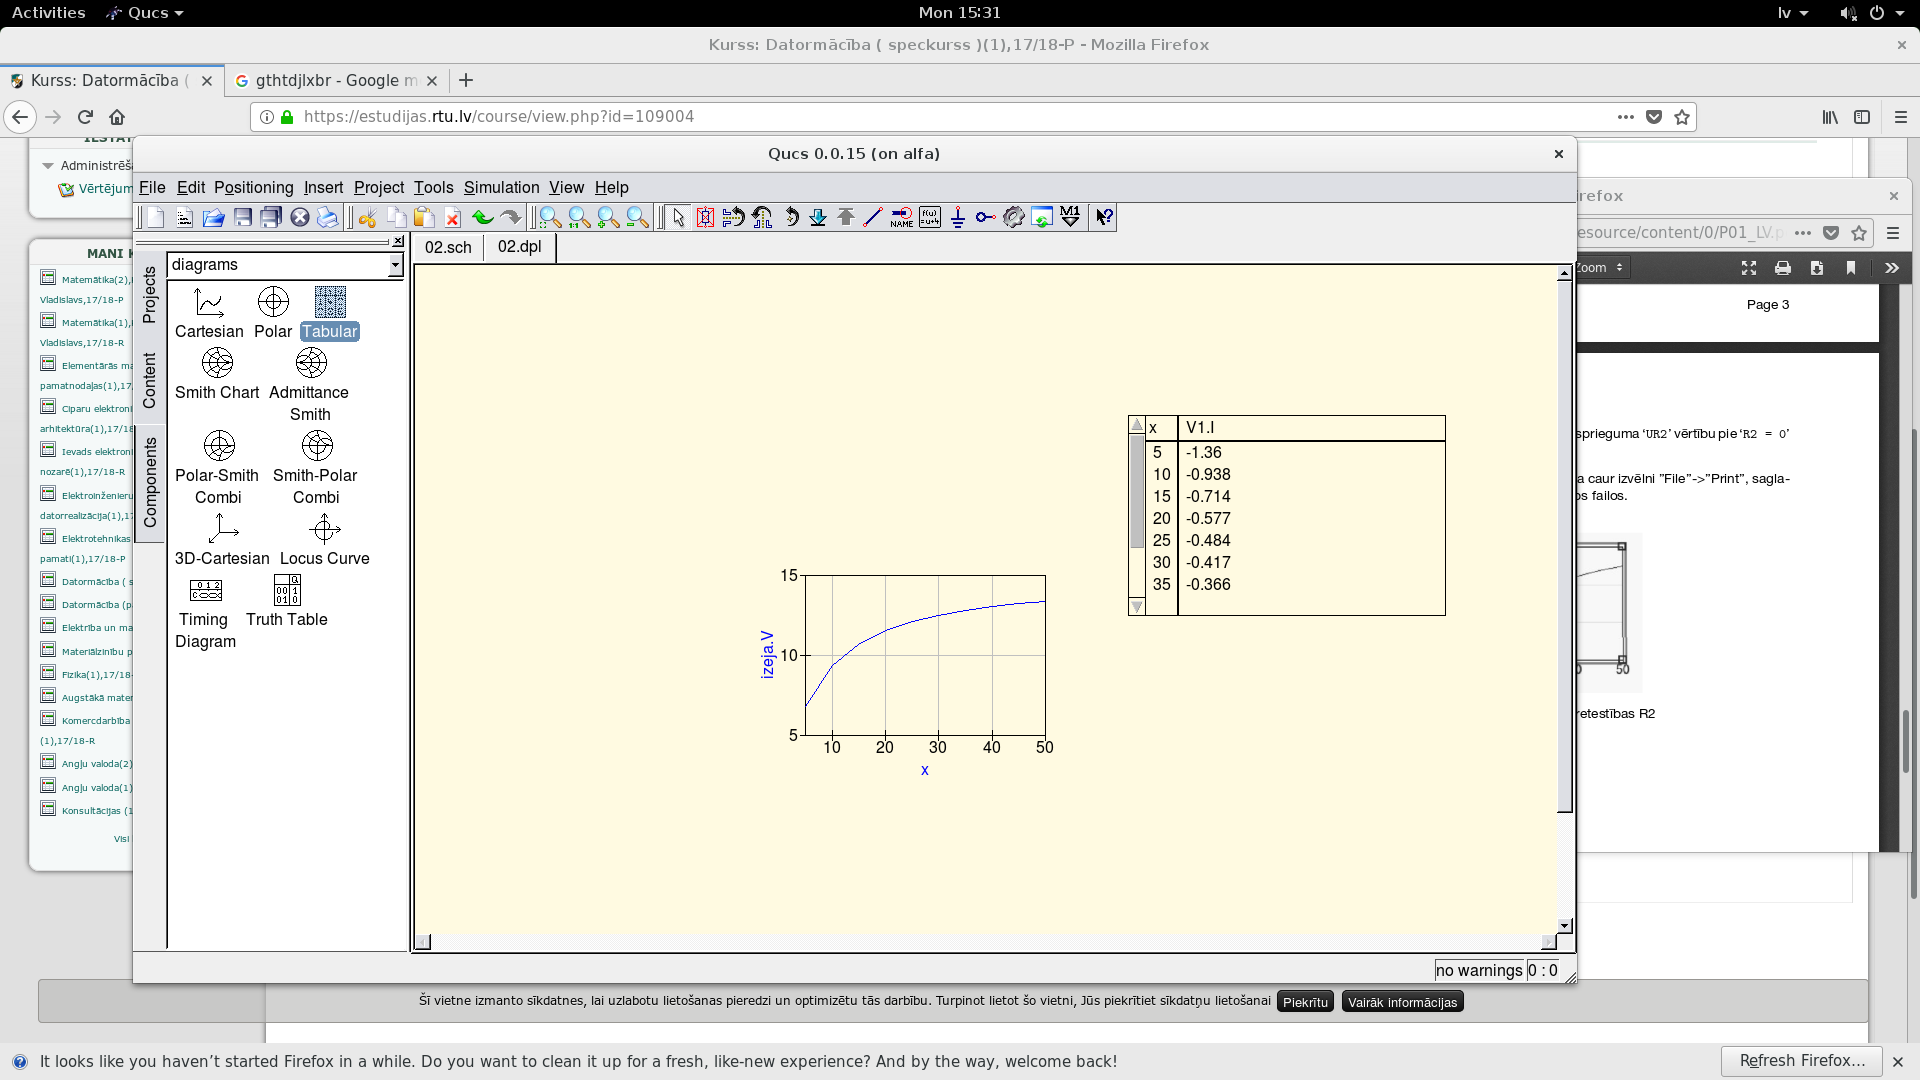
\includegraphics[scale=0.250]{10}}
\center{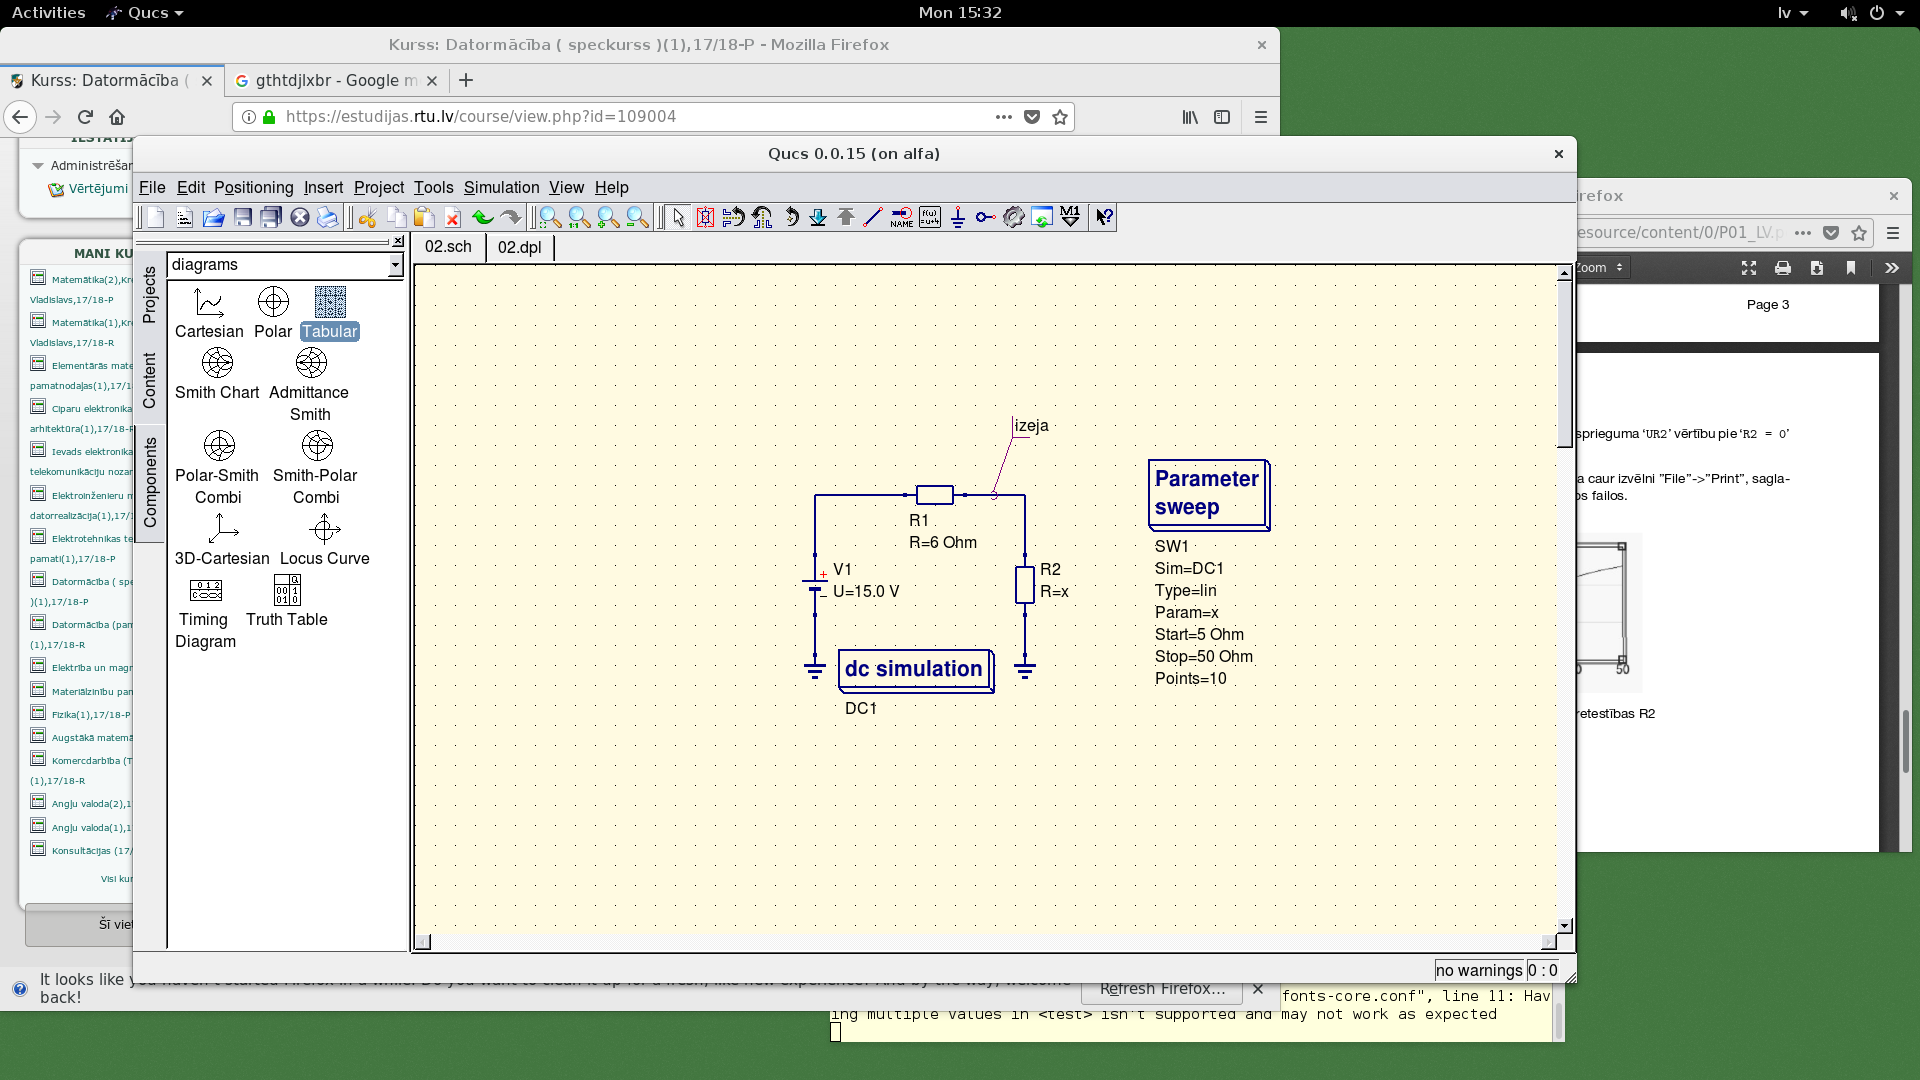
\includegraphics[scale=0.250]{20}}
\caption{Тестовый рисунок "Qucs palidziba"}
\label{fig:image}
\end{figure}
\section {Paskaidrojumus par katru attēlu un tabulu}
Attelus viegli darit kad mums ir viss iedot un ari tabulus.Bet bila daudz kodus kurie nau saprotams bet var darit. Grafiki ir tabulas ir un to var izdarit ar programmmam un vieglak.



\end{document}